\documentclass[../main.tex]{subfiles}
\graphicspath{{\subfix{../img/}}}
\newacronym
  {pren1}                % id
  {PREN 1}                % display name
  {Produktentwicklung 1}  % full acronym name
  
\newacronym
  {pren2}                % id
  {PREN 2}                % display name
  {Produktentwicklung 2}  % full acronym name

\newacronym
  {yaml}
  {YAML}
  {YAML Ain't Markup Language}

\newacronym
  {tof-sensor}
  {ToF-Sensor}
  {Time-of-Flight Sensor}

\newglossaryentry{h-brücke}{
    name={H-Brücke},
    description={
         Eine H-Brücke ist eine Schaltung, die es ermöglicht, einen Elektromotor in beide Richtungen zu betreiben, indem sie den Stromfluss durch den Motor umkehrt. Sie besteht aus vier Schaltern (meistens Transistoren oder MOSFETs), die in einer "H"-Form angeordnet sind. Die Schalter werden so gesteuert, dass der Motor entweder vorwärts, rückwärts oder gestoppt wird.
    }
}


\newglossaryentry{pwm}{
    name={PWM},
    description={
        PWM (Pulsweitenmodulation) ist eine Technik zur Steuerung der Leistung von elektrischen Geräten, wie Motoren oder LEDs, durch das schnelle Ein- und Ausschalten eines Signals. Dabei wird die Dauer, in der das Signal "ein" ist (die Pulsbreite), im Vergleich zur Gesamtdauer eines Zyklus (der Periode) variiert.
    }
}


\newglossaryentry{ir-fototransistor}{
    name={IR-Fototransistor},
    description={
        Ein Fototransistor ist ein Halbleiterbauteil, das Licht in elektrischen Strom umwandelt. Wenn Licht auf den Transistor trifft, verändert sich seine elektrische Leitfähigkeit, was zu einer Stromänderung führt. Ein Infrarot(IR)-Fototransistor reagiert speziell auf Infrarotlicht. 
    }
}


\newglossaryentry{i2c}{
    name={I\textsuperscript{2}C},
    description={
        Eine serielle Kommunikationsschnittstelle, die den Datenaustausch zwischen verschiedenen Komponenten wie Mikrocontrollern, Sensoren und Aktoren über nur zwei Leitungen ermöglicht: \textit{Serial Data Line} für die Datenübertragung und \textit{Serial Clock Line} für die Synchronisation. 
        Die I\textsuperscript{2}C-Schnittstelle unterstützt mehrere Geräte in einem Netzwerk und verwendet Adressen, um einzelne Komponenten anzusprechen.
    }
}


\newglossaryentry{uart}{
    name={UART},
    description={
        Abkürzung für \textit{Universal Asynchronous Receiver Transmitter}. 
        Eine Hardware-Komponente oder ein Kommunikationsprotokoll, das zur seriellen, asynchronen Datenübertragung verwendet wird. 
        UART ermöglicht die Kommunikation zwischen zwei Geräten, indem Daten über eine Sendeleitung (\textit{TX}) und eine Empfangsleitung (\textit{RX}) übertragen werden. Es erfordert keine gemeinsame Taktleitung und verwendet stattdessen Start- und Stoppbits zur Synchronisation. 
    }
}


\newglossaryentry{PLA}{
    name={PLA},
    description={
    Polymilchsäure   (PLA) ist ein biologisch   abbaubarer, thermoplastischer Kunststoff, der aus erneuerbaren Ressourcen wie Maisstärke oder Zuckerrohr hergestellt wird.
    }}

\begin{document}

\newpage
\section{Lösungskonzept}\label{lösungskonzept}

In diesem Kapitel wird das gewählte Lösungskonzept ''Simpel'' (siehe Anhang \ref{a3:loesungsvariante_Simpel}) näher erläutert. Wieso das Lösungskonzept ''Beweglich'' ausgeschieden ist, steht im Anhang \ref{a3:EntscheidLösungsvariante} beschrieben. Bei dem gewählten Konzept liegt der Schwerpunkt auf einer möglichst einfachen Lösung. Ein einfach konstruiertes System ist in der Regel robuster im Einsatz. In der Abbildung \ref{img:Konzept-Skizze_Fahrzeug} ist eine Skizze von dem gewählten Lösungskonzept ''Simpel'' zu sehen.

\begin{figure}[H]
\centering
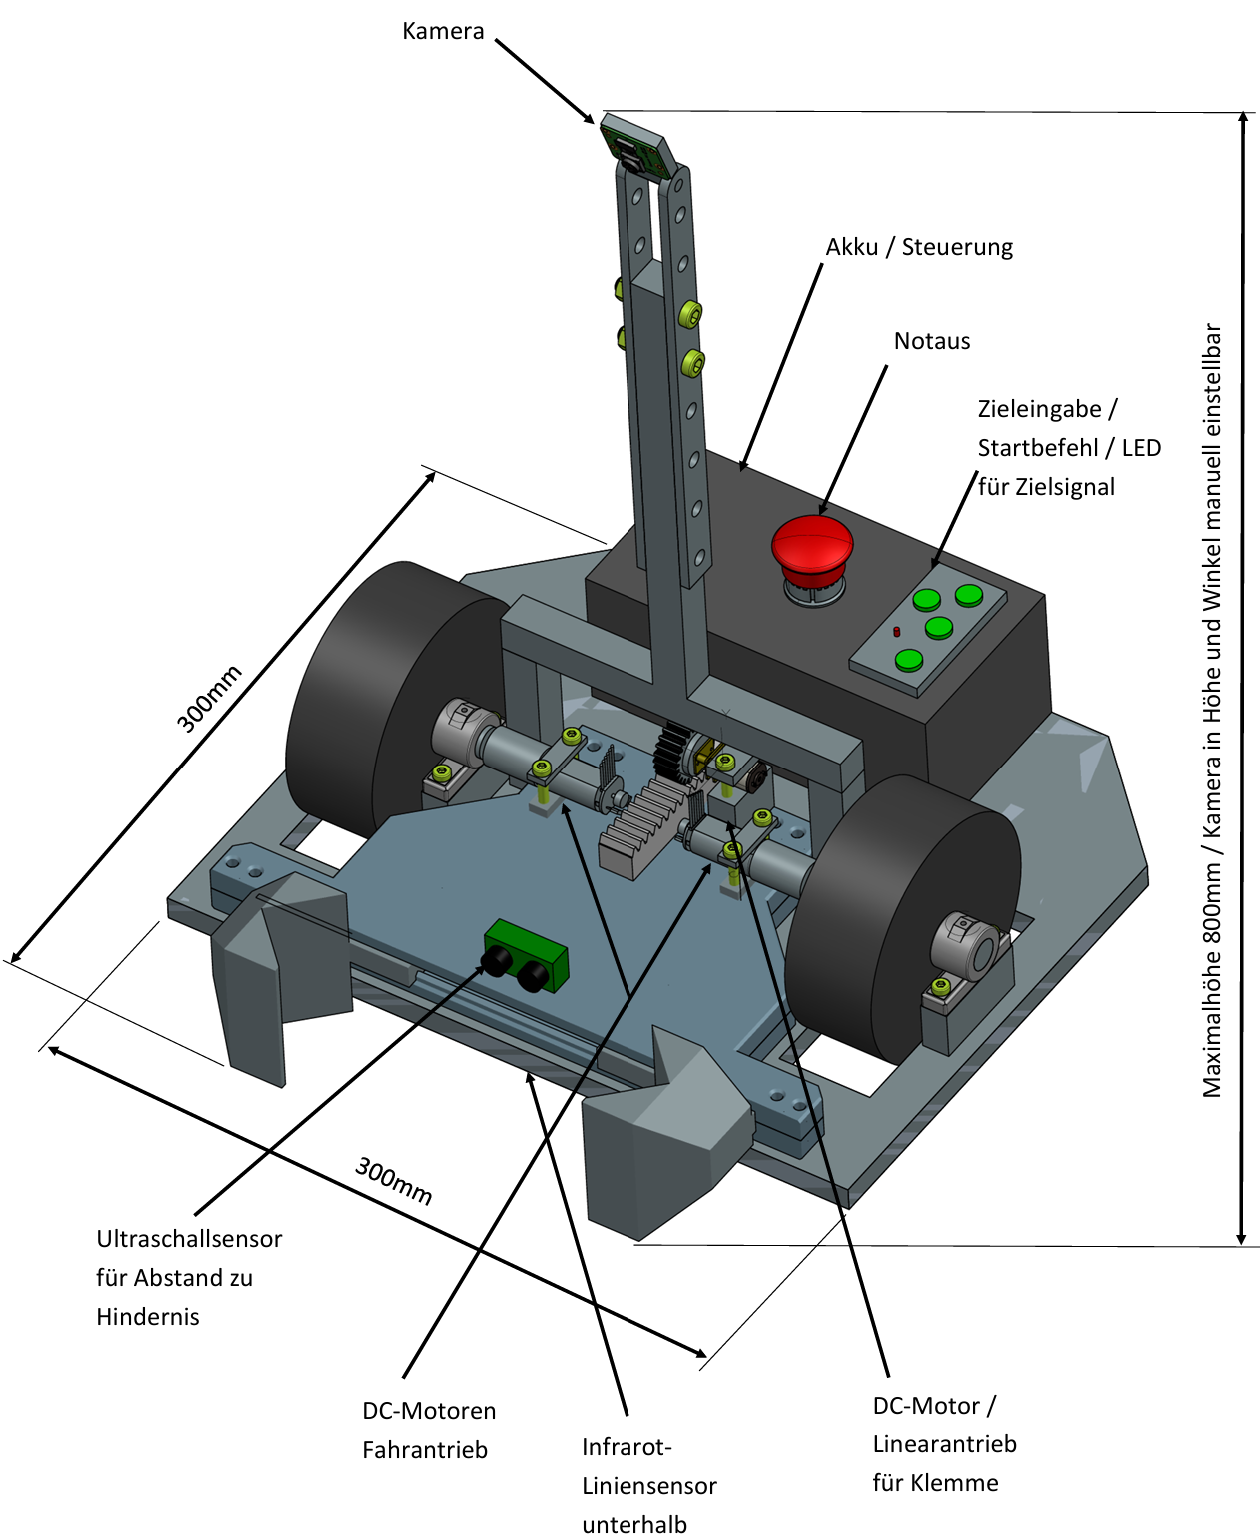
\includegraphics[width=0.85\linewidth]{Skizze Konzept beschriftet.png}
\caption{Skizze des Lösungskonzepts}
\label{img:Konzept-Skizze_Fahrzeug}
\end{figure}

\newpage
\subsection{Überblick}
Dieser Abschnitt dient dazu, der lesenden Person eine bessere Nachvollziehbarkeit über die Erarbeitung des gewählten Lösungskonzepts zu geben.
Alle detaillierte Informationen über die Erarbeitung des Lösungskonzepts und die weiteren Lösungsansätze sind im Anhang aufgeführt. Sie werden nicht im Hauptteil erwähnt.

Nach Erarbeitung der Anforderungsliste und zum Start der Konzeptfindung begann die Technologierecherche (siehe Anhang \ref{a2:technologierecherche}). Dafür ist die Aufgabenstellung in die verschiedenen Themengebiete Wegfindung (siehe Anhang \ref{a2:Wegfindung}), Objekterkennung (siehe Anhang \ref{a2:Objekterkennung}), Fortbewegung (siehe Anhang \ref{a2:Fortbewegung}), Hindernisbewältigung (siehe Anhang \ref{a2:Hindernisbewältigung}) und Antrieb und Orientierung (siehe Anhang \ref{a2:Antrieb_Orientierung}) unterteilt. Durch die Technologierecherche liegen eine grosse Anzahl an Lösungsmöglichkeiten vor. 

Für die Konzeptfindung (siehe Anhang \ref{a3:Konzeptfindung}) wird mit den Methodiken Nutzwertanalysen und morphologischer Kasten gearbeitet. In einer Vorauswahl ist das Gesamtkonzept in dieselben Teilfunktionen zerlegt, wie bei der Technologierecherche (siehe Anhang \ref{a3:Vorauswahl}). Jeder Lösungsansatz hat seine Vor- und Nachteile. Um diese bestmöglich zu vergleichen, werden in den Teilbereichen Fortbewegung (siehe Anhang \ref{a3:Fortbewegung}), Hardwaresteuerung (siehe Anhang \ref{a3:Hardware Steuerung}), Objekterkennung Software (siehe Anhang \ref{a3:Objekterkennung}), Wegfindung (siehe Anhang \ref{a3:Wegfindung}), Energiequelle (siehe Anhang \ref{a3:Energiequelle}) und der Hindernisaufnahme (siehe Anhang \ref{a3:Aufnahme_Hindernis}) Nutzwertanalysen durchgeführt. Dabei werden verschieden Kriterien gewichtet. Durch die Bewertung ist ersichtlich, welcher Lösungsansatz sich am besten eignet.

Die ausgewählten Lösungsansätze sind unter ihrer Teilfunktion im morphologischen Kasten aufgeführt (siehe Anhang \ref{morphologischer kasten}). Im morphologischen Kasten sind zwei verschiedene Lösungsversionen visualisiert. Es gibt eine Lösungsvariante ''Simpel'' (siehe Anhang \ref{a3:loesungsvariante_Simpel}) und eine Lösungsvariante ''Beweglich'' (siehe Anhang \ref{a3:loesungsvariante_beweglich}). Für die Entscheidung sind die Erkenntnisse aus den Nutzwertanalysen ausschlaggebend (siehe Anhang \ref{a3:EntscheidLösungsvariante}).
\newpage

\subsection{Aufbau}

Das Fahrzeug besitzt zwei Räder. Der Antrieb erfolgt mit DC-Motoren. Um das Fahrzeug zu balancieren, hat es am hinteren Fahrzeugende eine dritte Auflagefläche.

Die Raspberry Pi Module 3 Kamera befindet sich auf einem höhenverstellbaren Masten. Die Höhe der Kamera ist zwischen 40 und 60 Zentimeter manuell einstellbar. Der Winkel der Kamera ist ebenfalls manuell veränderbar. Somit kann die Kamera-Position im späteren Verlauf des Projektes einfach optimiert werden.

Zur Hindernisbewältigung befindet sich an der Vorderseite des Fahrzeugs ein Klemmmechanismus. Ein dritter DC-Motor zieht die beiden Klemmbacken des Mechanismus zusammen und hebt sie an. Der Mechanismus wird für die Hindernisbewältigung verwendet. Für die Abstandbestimmung zwischen Fahrzeug und Hindernis, befindet sich ein Ultraschallsensor zwischen den beiden Klemmbacken, auf dem Gehäuse. 

Die Motoren und Sensoren werden über ein TinyK22 Mikro-Controller-Board gesteuert. Das TinyK22, die Eingabeknöpfe sowie die Kamera sind an einem Raspberry Pi 5 Einplatinencomputer angeschlossen.

Ein LiPo-Akku stellt die Energieversorgung sicher (siehe Anhang \ref{a3:Energiequelle}).
Mit dem Notaus-Schalter kann die Energieversorgung zu allen Komponenten direkt unterbrochen werden.
In der Abblidung \ref{img:Blockschaltbild-Aufbau} ist der Aufbau visuell dargestellt.
\newline
\begin{figure}[H]
\centering
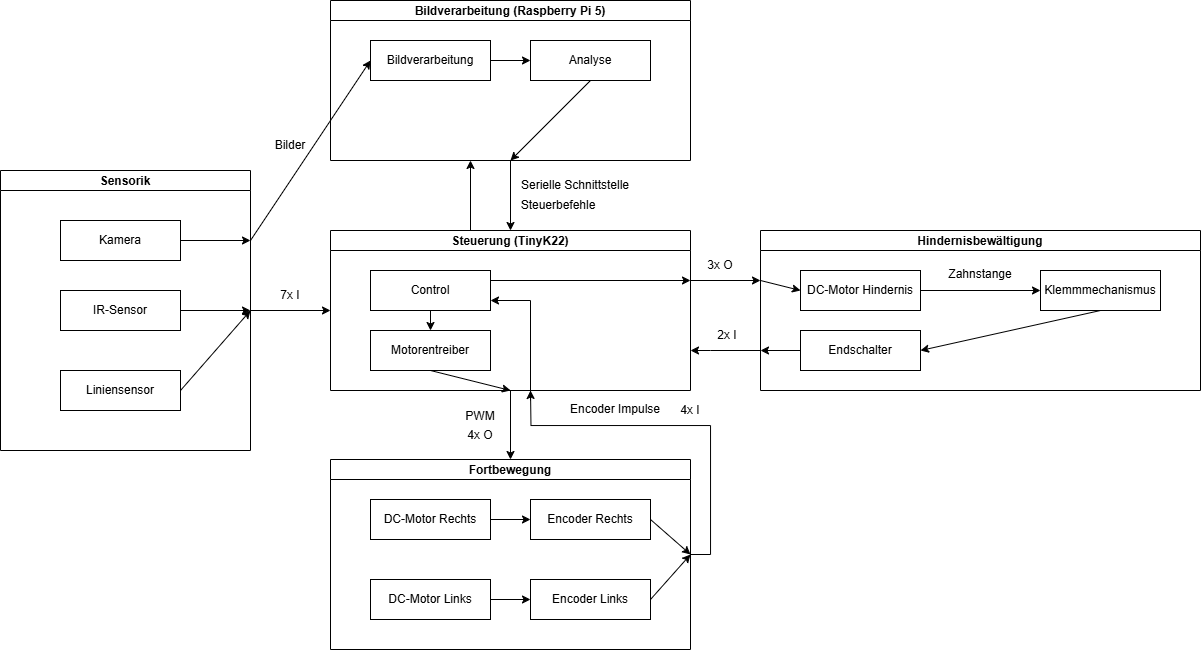
\includegraphics[width=1\textwidth]{img/lösungskonzpet/Blockschaltbild.png}
\caption{Blockschaltbild Aufbau}
\label{img:Blockschaltbild-Aufbau}
\end{figure}

\subsection{Ablauf}

Im Ablaufdiagramm (Abbildung \ref{img:ablaufdiagramm}) wird der Programmablauf des Fahrzeugs von Start bis Ziel aufgezeigt.

\begin{figure}[H]
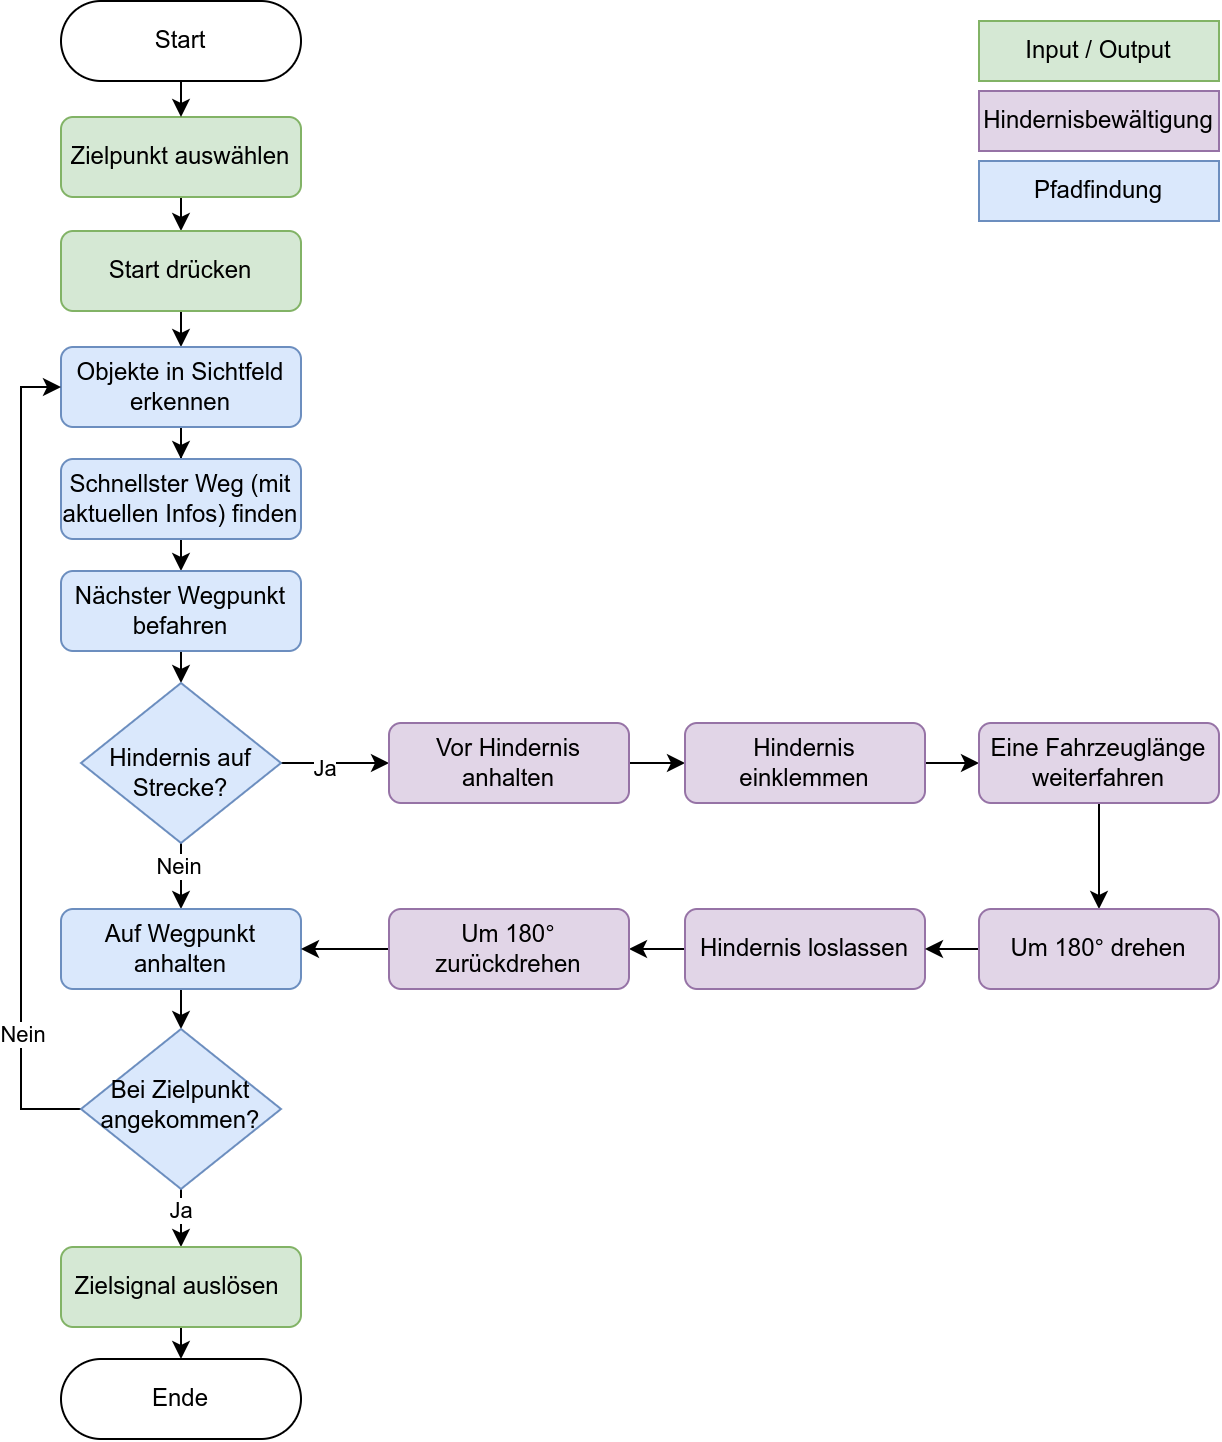
\includegraphics[width=0.9\textwidth]{img/lösungskonzpet/Ablaufdiagramm.png}
\caption{Ablaufdiagramm des Fahrzeug-Programms}
\label{img:ablaufdiagramm}
\end{figure}

\newpage
\subsection{Zielauswahl}
\imagefloat{img/lösungskonzpet/Skizzen/Zielauswahl.png}{Zielauswahl (Ausschnitt aus Abbildung \ref{img:Konzept-Skizze_Fahrzeug})}{0.3\textwidth}

Das Ziel des Fahrzeugs muss vor dem Start ausgewählt werden. Die Auswahlmöglichkeiten sind A, B oder C. Jede dieser Optionen ist über einen physischen Knopf am Fahrzeug wählbar ist.

Neben der Zielauswahl befindet sich der Startknopf des Fahrzeugs. Dieser funktioniert bloss, falls eine Zielauswahl vorliegt. Bei einer mehrfachen Zielauswahl wird das zuletzt gewählte Ziel angesteuert.

Sobald das Fahrzeug das Ziel erreicht, leuchtet die LED neben der Starttaste auf.

\subsection{Fortbewegung} 

Die Fortbewegung wird nach dem Prinzip Roomba realisiert: Der Aufbau besteht aus zwei einzeln angetriebene Räder und einem Stützelement. Es handelt sich dabei um ein ähnliches System, wie es bei Staubsauger-Robotern vorkommt. Die beiden Räder können unabhängig in beide Drehrichtungen angesteuert werden. Das ermöglicht eine Wendung an Ort und Stelle. Die beiden Räder sind in Längsrichtung zentrisch angeordnet. Dadurch kann sich das Fahrzeug um den eigenen Mittelpunkt drehen, ohne dass ein Versatz entsteht(siehe Anhang \ref{a3:Fortbewegung}).

Als Antriebsmotoren werden DC-Motoren verwendet. Eine \gls{h-brücke} dient als Motorentreiber. Die Geschwindigkeit ist über ein \gls{pwm}-Signal ansteuerbar. Jeder Motor verfügt über einen Encoder. Er überwacht, dass beide Motoren die gleiche Anzahl an Umdrehungen ausführen. Das TinyK22 steuert die Motoren über die \gls{h-brücke} (siehe Anhang \ref{a3:Hardware Steuerung}). Weitere Details sind im Anhang \ref{a3:Fahrantrieb} und \ref{a3:Sensorik:Positionsabfrage} vorhanden.

Die Steuerung des Fahrzeugs erfordert eine präzise Kommunikation zwischen den Baugruppen. Während die Motoren und die H-Brücke die Fortbewegung des Fahrzeugs sicherstellen, übernimmt das TinyK22 die Steuerung der Antriebssysteme und die Verarbeitung der Sensordaten. Um eine koordinierte Navigation zu ermöglichen, kommuniziert das TinyK22 kontinuierlich mit dem Raspberry Pi, der die übergeordnete Planung und die Bildverarbeitung übernimmt.
\newpage
Das TinyK22 ist über eine \Gls{uart}-Schnittstelle mit dem Raspberry Pi verbunden (siehe Abbildung \ref{img:UART_Physisch}). In der Abbildung \ref{img:UART_Signalablauf} ist der Datenaustausch zwischen dem Raspberry und dem TinyK22 ersichtlich. Als erstes  analysiert der Raspberry Pi mit der Kamera den besten Punkt. Anschliessend teilt er dem TinyK22 mit, um welchen Winkel das Fahrzeug sich drehen muss. Der Liniensensor verifiziert den korrekten Sandort über einer Linie. Wird die Linie nicht erkannt, sucht das System die Linie durch Drehungen im Bereich von ±15 Grad. Sobald die Linie verifiziert ist, meldet das TinyK22 dem Raspberry Pi, wie weit sich das Fahrzeug gedreht hat. Dies benötigt das Raspberry Pi, um die relative Position der Kamera zu bestimmen. Jetzt folgt das Fahrzeug der Linie mithilfe des Liniensensors. Erkennt der Liniensensor eine breitere Linie, also einen Punkt, informiert das TinyK22 den Raspberry Pi und stoppt das Fahrzeug. Der Vorgang beginnt erneut. Sobald das Fahrzeug den Zielpunkt erreicht, signalisiert der Raspberry Pi dies dem TinyK22. Das TinyK22 lässt anschliessend die LED blinken.

\begin{figure}[H]
\centering
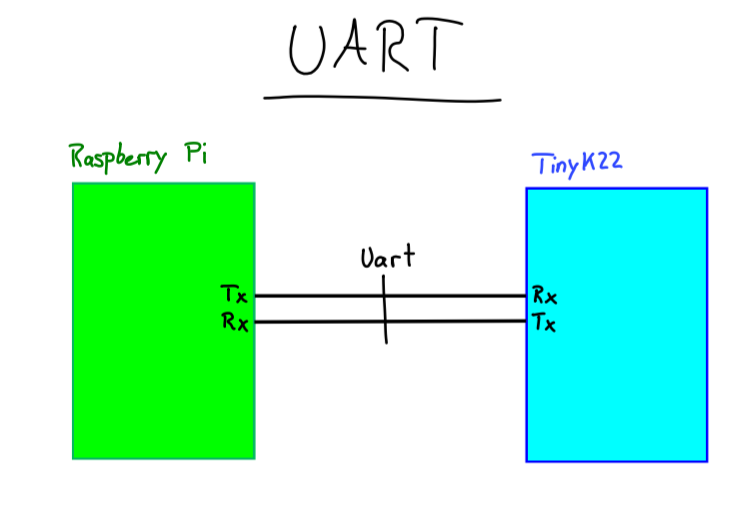
\includegraphics[width=0.6\textwidth]{img/lösungskonzpet/Skizzen/Uart_Physisch.png}
\caption{\Gls{uart} Physische Verbindung}
\label{img:UART_Physisch}
\end{figure}

\begin{figure}[H]
\centering
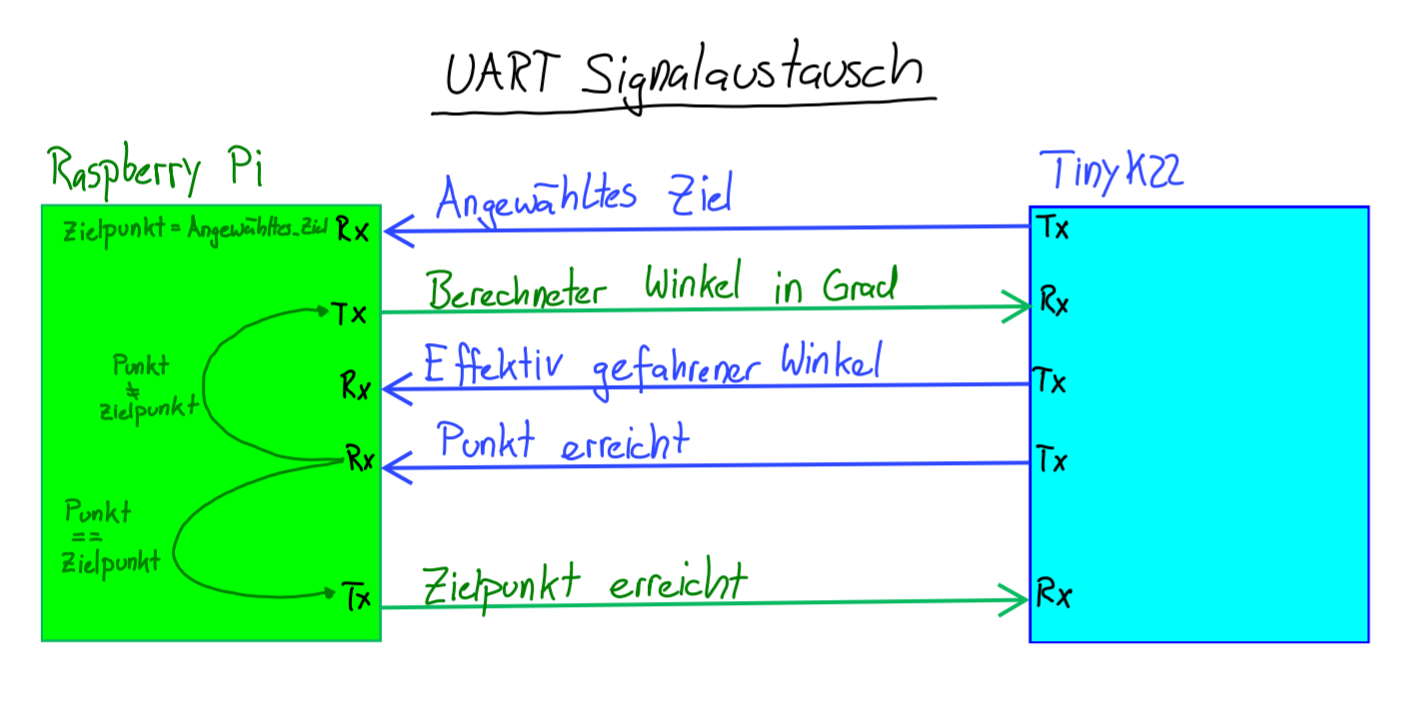
\includegraphics[width=0.8\textwidth]{img/lösungskonzpet/Skizzen/Uart_Signalaustausch.png}
\caption{\Gls{uart} Signalablauf}
\label{img:UART_Signalablauf}
\end{figure}




\newpage

\subsection{Wegfindung}

Der schnellste Weg ins Ziel wird mithilfe des Dijkstra-Algorithmus berechnet (siehe Anhang \ref{a3:Wegfindung}). Dabei wird das vorgegebene Liniennetz als gewichteter Graph in der Software gespeichert. Die Wegpunkte werden als Knoten und die Linien als Kanten betrachtet. Ursprünglich besitzen alle Kanten eine einheitliche Gewichtung. Sobald die Kamera neue Informationen über die Strecke erfasst (siehe Kapitel \ref{sub:Objekterkennung}), wird der Graph entsprechend aktualisiert. Der kürzeste Weg wird basierend auf der aktuellen Position neu berechnet.

Je nach neu erhaltener Information werden folgende Anpassungen am Graphen vorgenommen: \begin{itemize} 
  \item Pylon auf Wegpunkt erkannt: Der Wegpunkt (Knoten) wird aus dem Graphen entfernt.
  \item Linie wurde entfernt: Die Linie (Kante) wird aus dem Graphen entfernt. 
  \item Hindernis auf Linie erkannt: Die Linie (Kante) erhält eine höhere Gewichtung.
\end{itemize}

\subsubsection{Objekterkennung} \label{sub:Objekterkennung}
Die weitwinklige Raspberry Pi Module 3 Kamera macht die Bilder für die Objekterkennung. Pylonen, Hindernisse und Wegpunkte sollen erkannt werden. Als Software kommt YOLO zum Einsatz (siehe Anhang \ref{a3:Objekterkennung}). Die erkannten Objekte werden für die Wegfindung genutzt. Bereits zu Beginn wird versucht, möglichst viele Objekte zu erfassen und auszuwerten. Da ein vollständiges und korrektes Ergebnis jedoch nicht garantiert ist, wird die Objekterkennung bei jedem Wegpunkt nochmals durchgeführt. 

\subsection{Hindernisbewältigung}
Der Ultraschallsensor überwacht kontinuierlich, ob sich ein Hindernis auf der Linie befindet (siehe Anhang \ref{a3:Objekterkennung_Sensor}). Ab einer Entfernung von 30 cm ist ein Hindernis erkennbar. Das Fahrzeug hält an, sobald das Hindernis sich zwischen den zwei seitlichen Klemmbacken befindet. Danach wird der DC-Motor angesteuert, welcher das Hindernis greift und gleichzeitig anhebt. Die genauen Details zu dieser Konstruktion befinden sich im Anhang \ref{a3:Hindernisbewältigungsantrieb} und \ref{a3:Aufnahme_Hindernis}.
Das Fahrzeug fährt anschliessend eine Fahrzeuglänge vor, wobei die Encoder die Fahrdistanz überwacht. Danach dreht sich das Fahrzeug um 180 Grad, und der Motor löst die Klemmen. Das Fahrzeug entfernt sich nun so weit vom Hindernis, bis es sich ohne Kollisionsgefahr um 180 Grad zurückdrehen kann. Abschliessend fährt das Fahrzeug mithilfe des Liniensensors entlang der Linie zum nächsten Punkt (siehe Abbildung \ref{img:Skizze_Hindernisbewältigung}).

\begin{figure}[H]
\centering
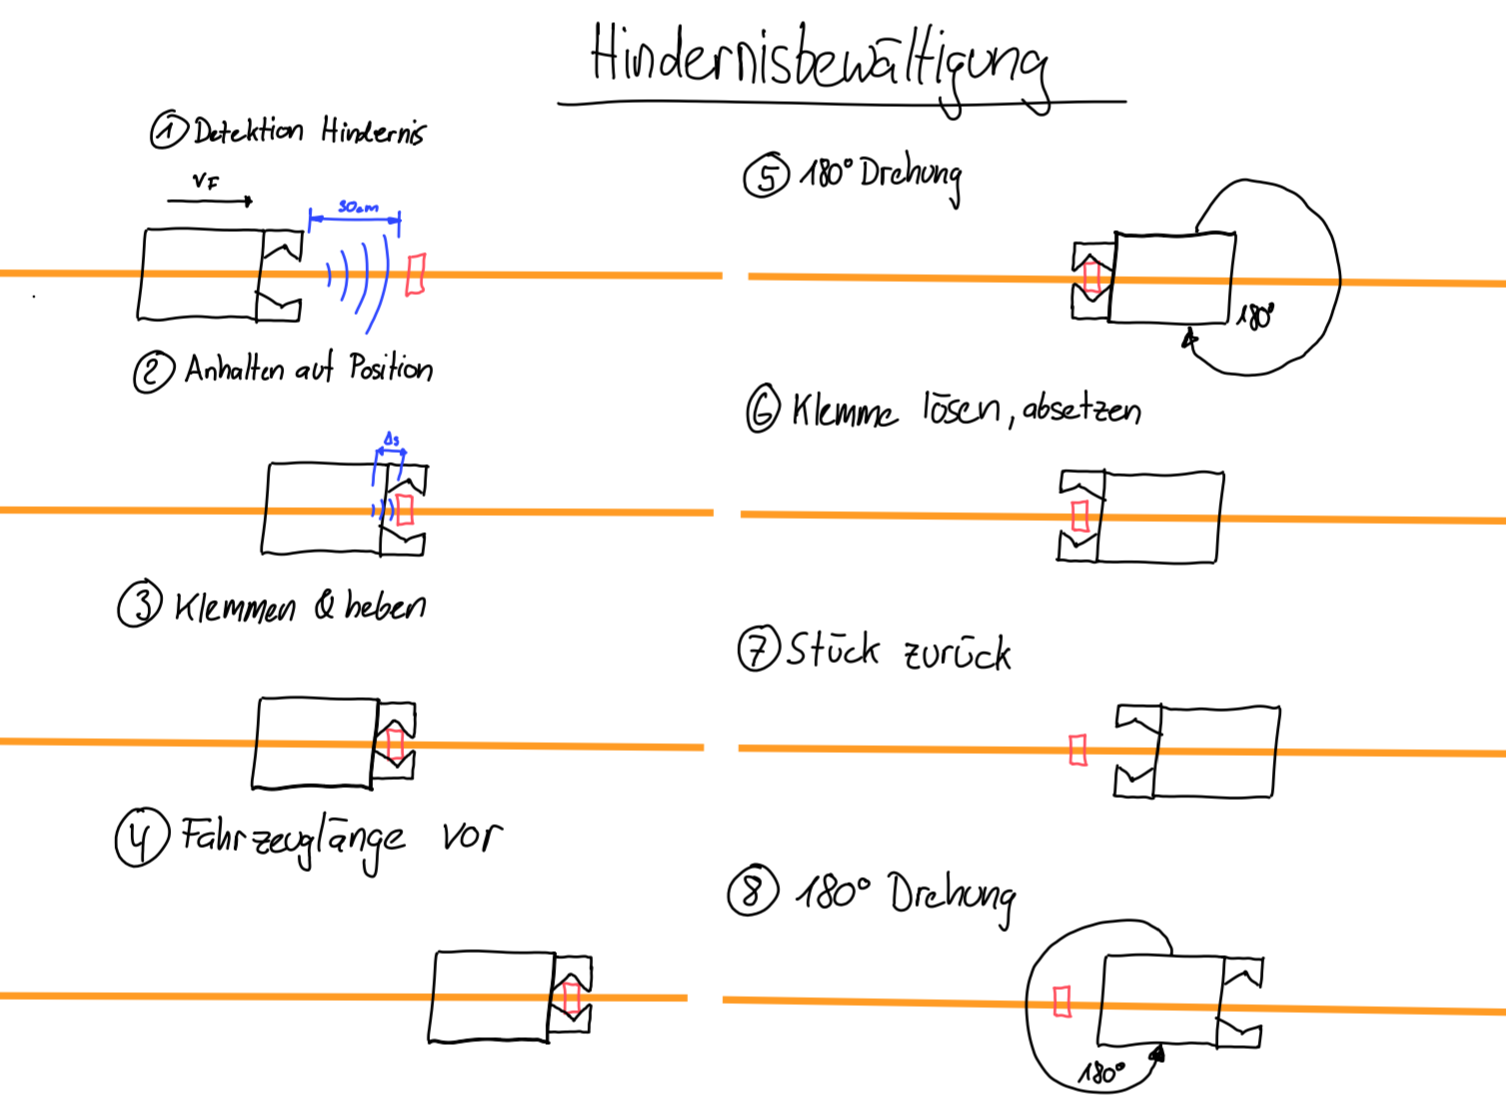
\includegraphics[width=0.7\textwidth]{img/lösungskonzpet/Skizzen/Skizze_Hindernisbewältigung.png}
\caption{Ablauf der Hindernisbewältigung}
\label{img:Skizze_Hindernisbewältigung}
\end{figure}


\subsubsection{Klemmmechanismus}

Zu Beginn des Projekts waren die Toleranzen für die Platzierung der Hindernisse seitens der Dozierenden noch sehr gross: Seitlich waren Abweichungen von bis zu 2 cm möglich (siehe Anforderungskatalog in Kapitel \ref{sec:anforderungsliste}). Seit dem 25. Oktober wurde diese Toleranz jedoch auf lediglich 5 mm reduziert. Unser Greifsystem erfüllt weiterhin die verschärften Anforderungen. Die ursprüngliche Toleranz von 2 cm wurde bewusst nicht angepasst, da sie uns bei der Messung der Genauigkeit einen grösseren Spielraum bietet.

Der Klemmmechanismus, welcher in Punkt 3 und 6 in der Abbildung \ref{img:Skizze_Hindernisbewältigung} benötigt wird, erfüllt mehrere Funktionen.

\begin{enumerate}
    \item Greifen
    \item Anheben
    \item Senken
    \item Loslassen
\end{enumerate}

Alle Funktionen werden mithilfe eines DC-Motors ausgeführt. Das Design ist in den Abbildungen \ref{fig:greifarm_oben} und \ref{fig:greifarm_unten} ersichtlich.
\newline

Zusätzlich soll die Konstruktion helfen, Fehler bei der Messung zu korrigieren.
\begin{enumerate}
    \item Korrektur Winkel (bis zu 15°, siehe Rechnung für Design in Anhang \ref{loes:winkel_verschiebung})
    \item Korrektur Distanz (bis zu 2.25 cm, siehe Rechnung für Design in Anhang \ref{loes:winkel_verschiebung})
    \item Korrektur Offset (bis zu 2 cm, siehe Definition für Design in Anhang \ref{loes:abstand_klemmen})
\end{enumerate}

\begin{figure}[H]
    \centering
    % Erste Minipage für das obere Bild
    \begin{minipage}[t]{0.45\textwidth}
        \centering
        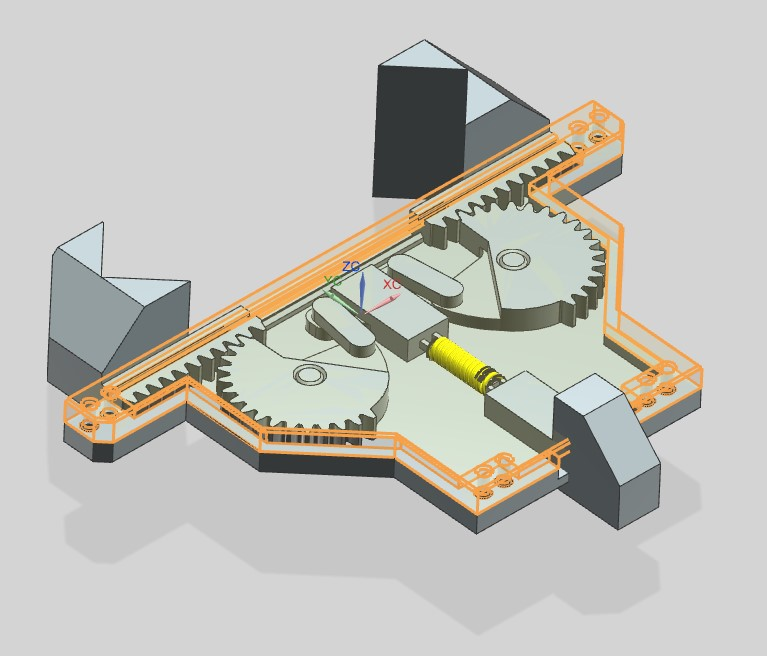
\includegraphics[height=6cm]{img/lösungskonzpet/hindernissaufnahme/Greifarm_oben.jpg}
        \caption{Klemm- \& Hebemechanismus von oben}
        \label{fig:greifarm_oben}
    \end{minipage}
    \hfill
    % Zweite Minipage für das untere Bild
    \begin{minipage}[t]{0.45\textwidth}
        \centering
        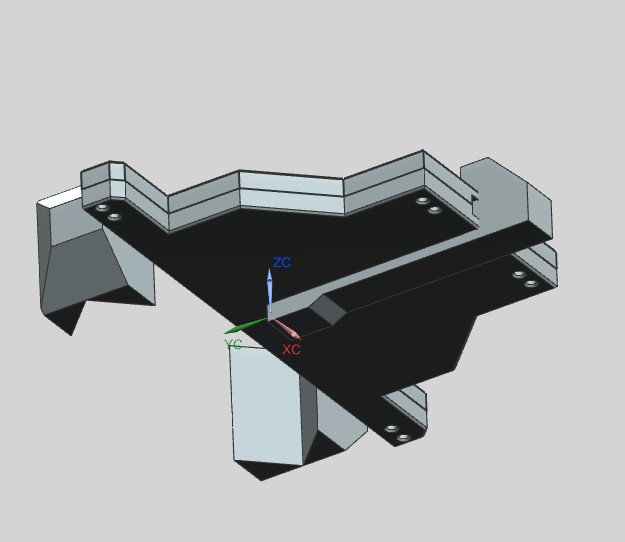
\includegraphics[height=6cm]{img/lösungskonzpet/hindernissaufnahme/Greifarm_unten.jpg}
        \caption{Klemm- \& Hebemechanismus von unten}
        \label{fig:greifarm_unten}
    \end{minipage}
\end{figure}
Die Abbildung \ref{fig:greifarm_oben} zeigt den Klemmmechanismus. Er wird durch Zahnräder angetrieben, welche wiederum von einem linearen Mechanismus bewegt werden, um gleichzeitig den Hebemechanismus auszulösen. Die Feder (Gelb in Abbildung \ref{fig:greifarm_oben} ersichtlich) sorgt dafür, dass sobald die nötige Griffkraft erreicht ist, weiterhin die Bewegung für den Hebemechanismus machbar ist. In der Abbildung \ref{fig:greifarm_unten} ist der Hebemechanismus zu sehen. Er drückt sich von einer nicht im Bild sichtbaren Plattform ab. An den Rändern befinden sich acht Löcher, von denen werden vier für Schrauben und die anderen vier für Führungen genutzt. Damit ist eine kontrollierte Anhebung des Hindernisses durch den Mechanismus sichergestellt.
Der DC-Motor, der den gesamten Mechanismus antreibt, ist am Gehäuse angebracht.
Der abgebildete Mechanismus ist zu Testzwecken für die Bedienung von Hand ausgelegt. Die Tests des Mechanismus sind im Kapitel \ref{sec:hardware_greifarm} ersichtlich.

\subsection{Materialwahl}
Die Materialwahl für den Klemm- \& Hebemechanismus sowie das \enquote{Chassis} ist essenziell. Nicht nur, um die Funktion korrekt zu erfüllen, sondern überwiegend, um Gewicht einzusparen. Aufgrund der Komplexität, der genauen Geometrie und geringer Belastungen, wurde für den Klemm- \& Hebemechanismus 3D-Druck ausgewählt. Voraussichtlich wird PLA-Filament oder ein festeres Filament eingesetzt. Da das Gewicht der Komponenten auf dem Chassis liegt, wird Aluminium verwendet. Holz hat eine viermal geringeren Dichte und ist ebenfalls geeignet. Da jedoch die Erfahrungen im Team sowie die Ausstattung der Werkstatt auf Metalle ausgerichtet sind, ist die Entscheidung auf Aluminium gefallen. Die Wahl der Materialien ist vorläufig definiert, muss jedoch zu einem späteren Zeitpunkt getestet werden.



\subsection{Prototyping Ergebnisse}
In diesem Kapitel werden die Ergebnisse verschiedener Tests vorgestellt. Die Ergebnisse sind entscheidend für das entstandene Lösungskonzept.
Die ausführlichen Berichte zu den durchgeführten Tests befinden sich im Anhang \ref{a4:prototyping}.

\subsubsection{Klemm- \& Hebemachanismus} \label{sec:hardware_greifarm}
Um das allgemeine Funktionsprinzip zu testen und Verbesserungen am Klemm- und Hebemechanismus vorzunehmen, wurde ein Prototyp mit dem 3D-Drucker hergestellt (siehe Abbildung \ref{fig:hardware_test_fertig}). Bei dem Zusammenbau und Funktionstest wurden diverse Erkenntnisse gewonnen:

\begin{enumerate}
    \item Funktionalität des Klemmmechanismus:
    \begin{itemize}
        \item Der Klemmmechanismus kann das Hindernis klemmen.
        \item Der Winkel für die Klemmbacken funktioniert einwandfrei.
        \item Die Führung der Klemmbacken muss vergrößert werden, da Schrumpfungseffekte durch 3D-Druck auftreten (siehe Abbildung \ref{fig:hardware_test_klemmen_gleiten}).
    \end{itemize}
    \item Platz- und Offset-Probleme:
    \begin{itemize}
        \item Zwischen den Klemmbacken ist nicht genügend Platz vorhanden, die Offset-Reserve fehlt.
    \end{itemize}
    \item Probleme mit dem Hebemechanismus:
    \begin{itemize}
        \item Der Hebemechanismus funktioniert nicht, da keine Führung für die Feder vorhanden ist (siehe Abbildung \ref{fig:hardware_test_schieber}).
        \item Für die lineare Bewegung fehlt eine geeignete Führung.
    \end{itemize}
    \item Probleme mit Zahnrädern und Verbindungen:
    \begin{itemize}
        \item Die Zahnräder reiben am Gehäuse. Der Luftspalt zwischen Zahnrad und dem Gehäuse muss vergrössert werden.
        \item Die Verbindungsstücke zwischen Schieber und Zahnrädern müssen länger sein.
    \end{itemize}
    \item Fertigungsprobleme:
    \begin{itemize}
        \item Alle Löcher sind zu klein aufgrund von Schrumpfungseffekten beim 3D-Druck (siehe Abbildung \ref{fig:hardware_test_loecher}).
    \end{itemize}
    \item Allgemeine Verbesserungsvorschläge:
    \begin{itemize}
        \item Für ein besseres Verhalten des gesamten Systems muss Silikonspray zum Einsatz kommen.
    \end{itemize}
\end{enumerate}
\begin{figure}[H]
    \centering
    \begin{minipage}[t]{0.45\textwidth}
        \centering
        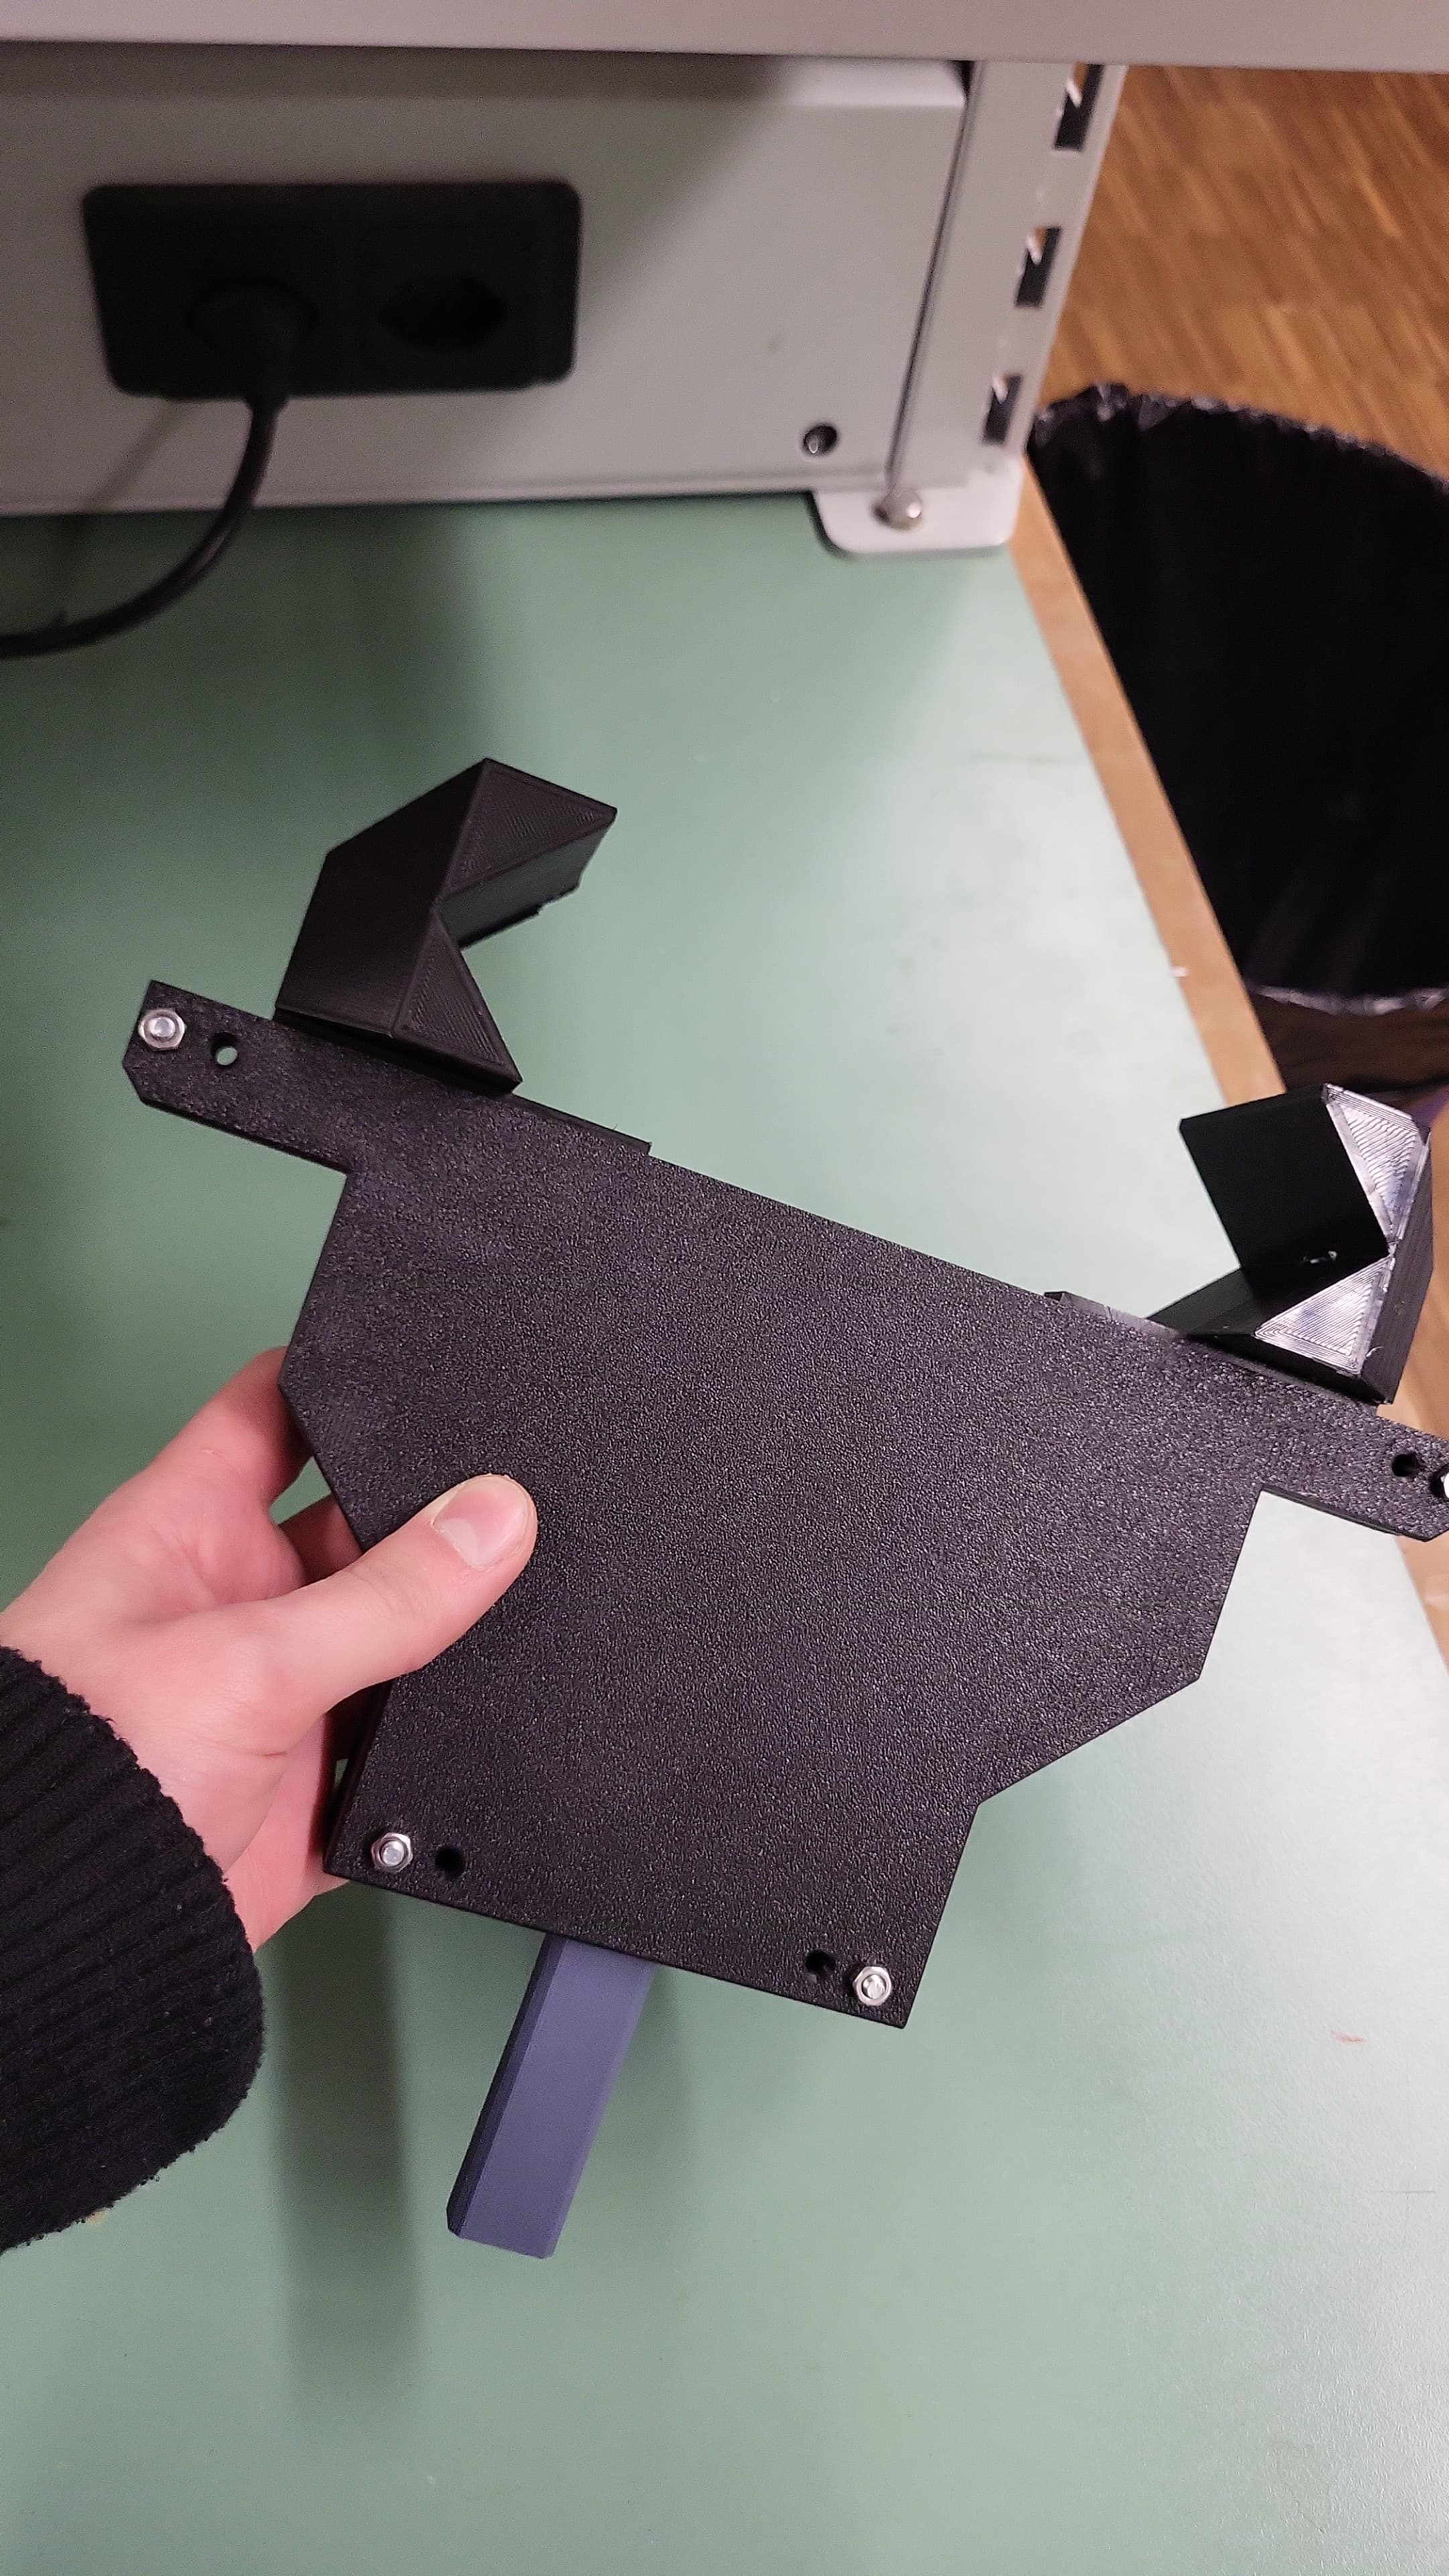
\includegraphics[height=9cm]{img/greifarmtest/prototyp_test_fertig.jpeg}
        \caption{Prototyp von Aussen}
        \label{fig:hardware_test_fertig}
    \end{minipage}%
    \hfill
    \begin{minipage}[t]{0.45\textwidth}
        \centering
        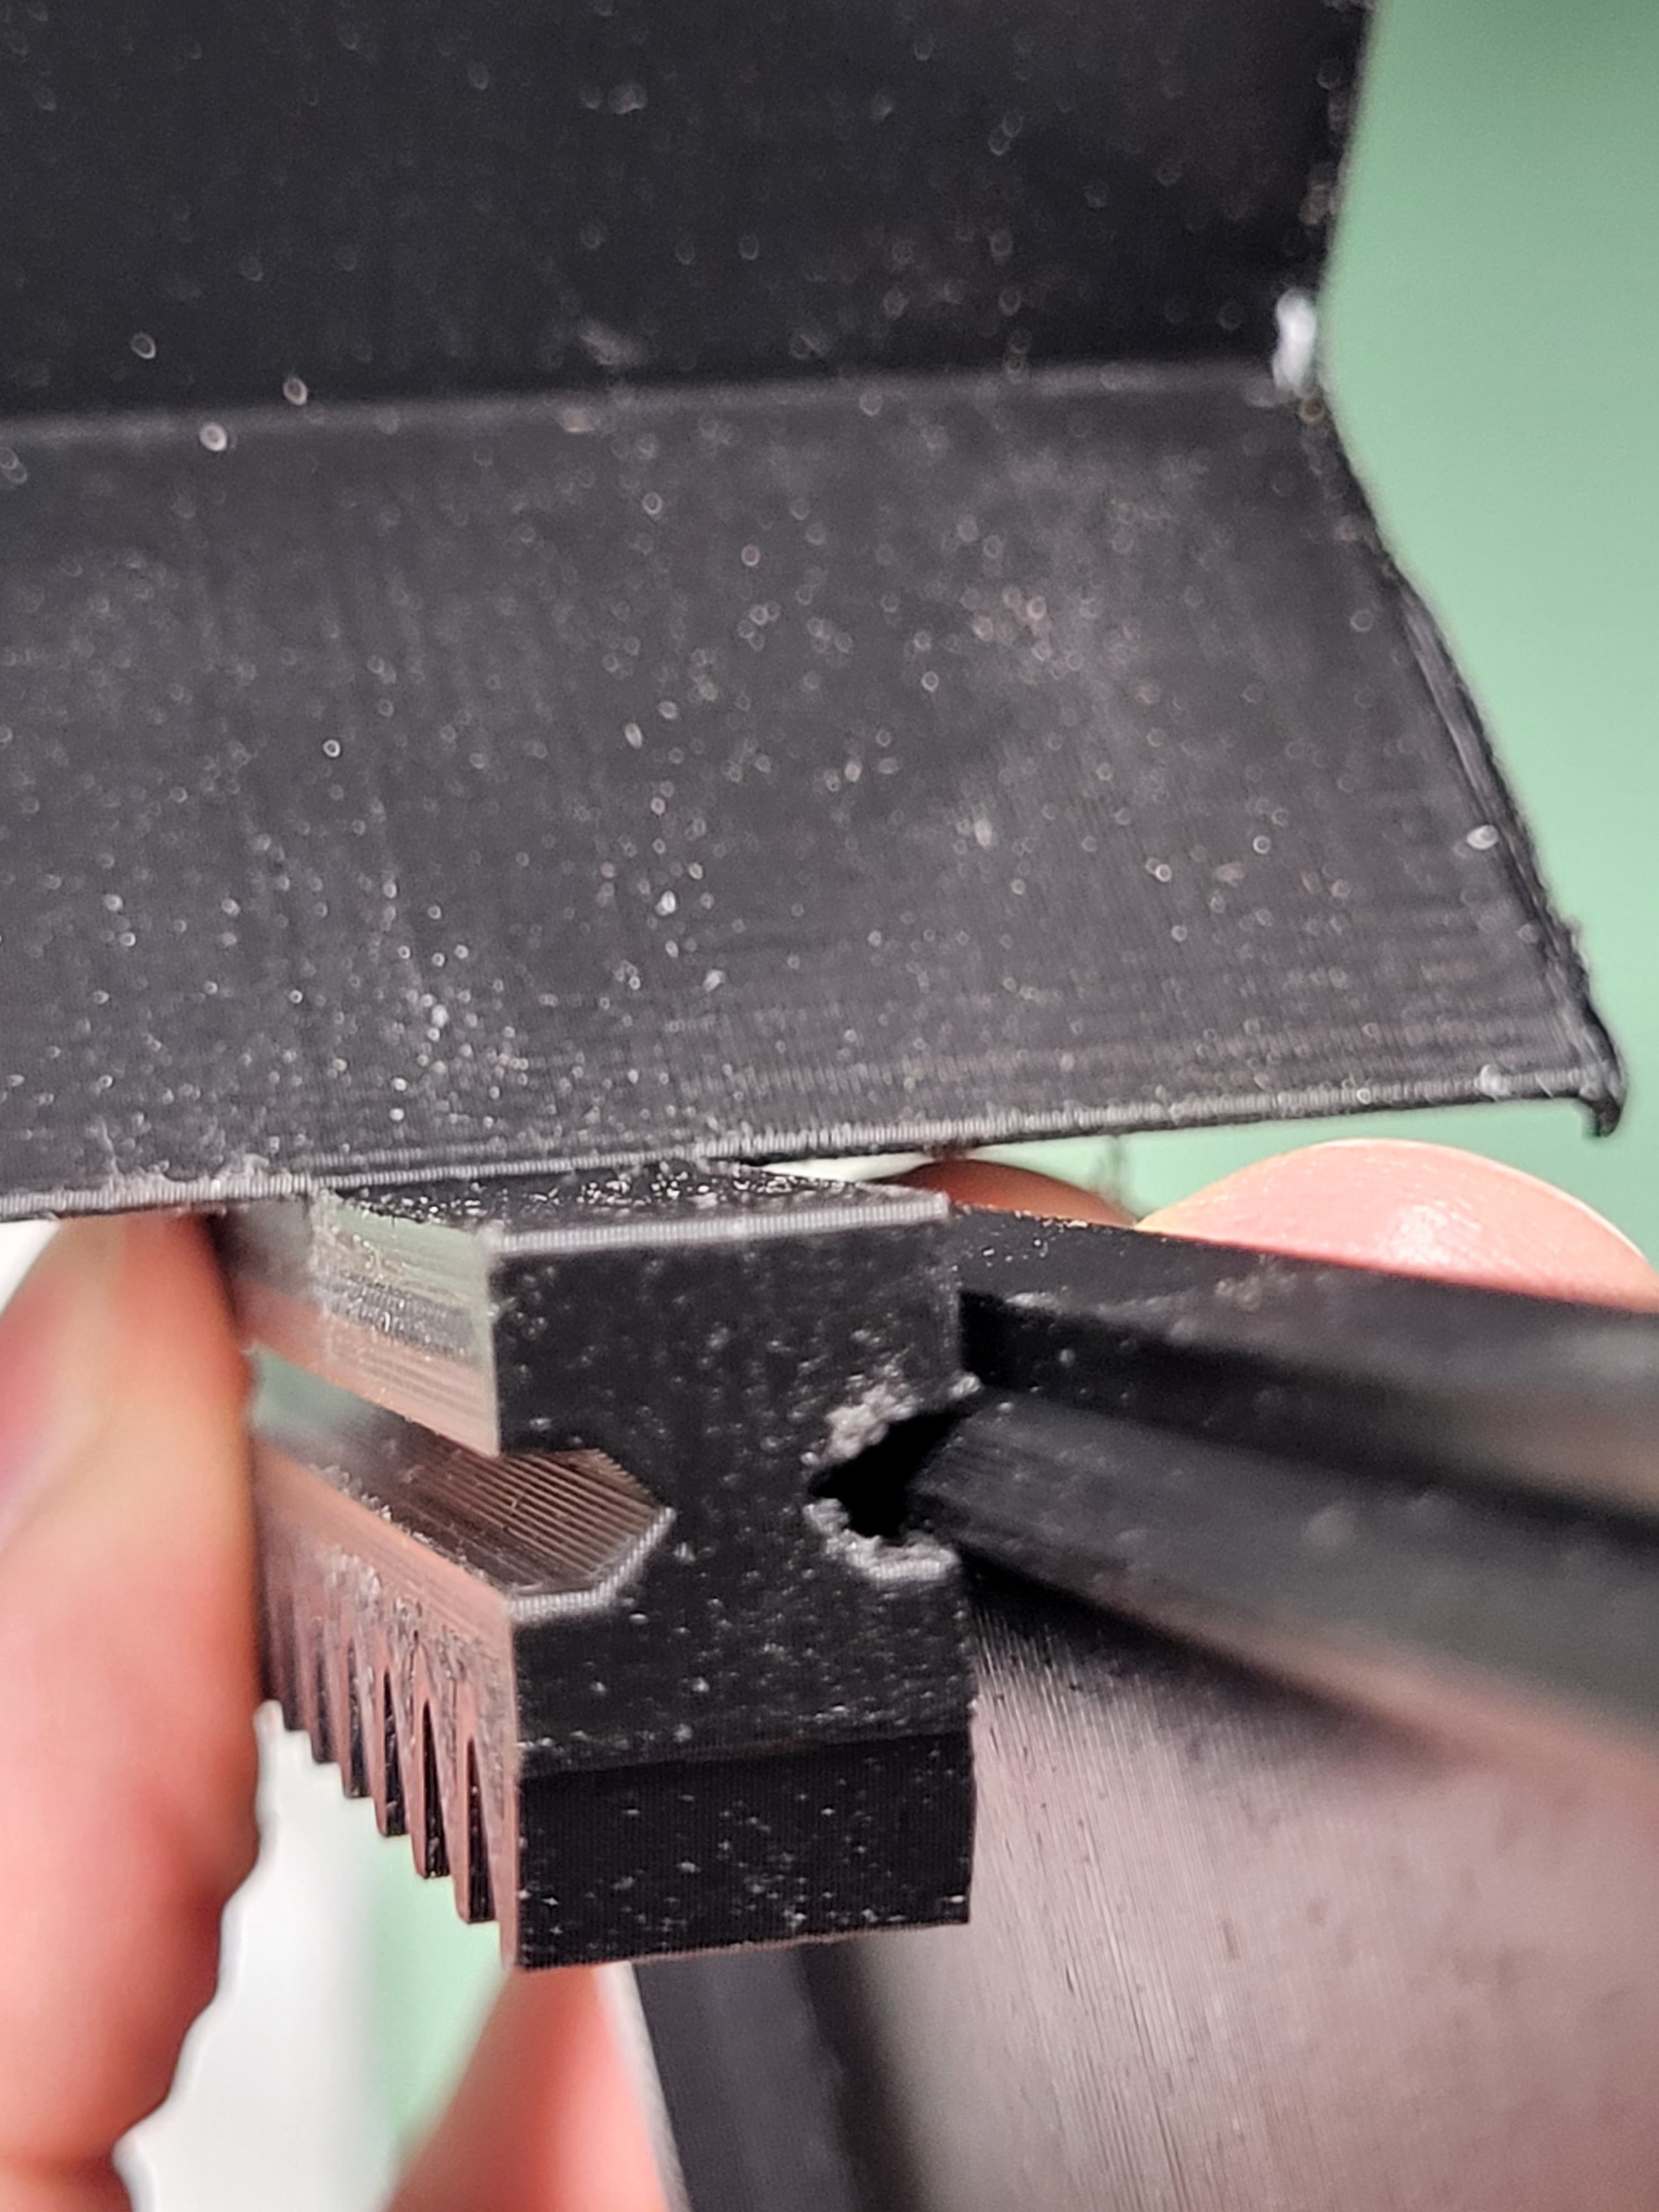
\includegraphics[height=9cm]{img/greifarmtest/prototyp_test_klemmen_gleiten.jpeg}
        \caption{Schrumpfungseffekte 3D-Druck: Führung der Klemmbacken passen nicht}
        \label{fig:hardware_test_klemmen_gleiten}
    \end{minipage}
\end{figure}

\begin{figure}[H]
    \centering
    \begin{minipage}[t]{0.45\textwidth}
        \centering
        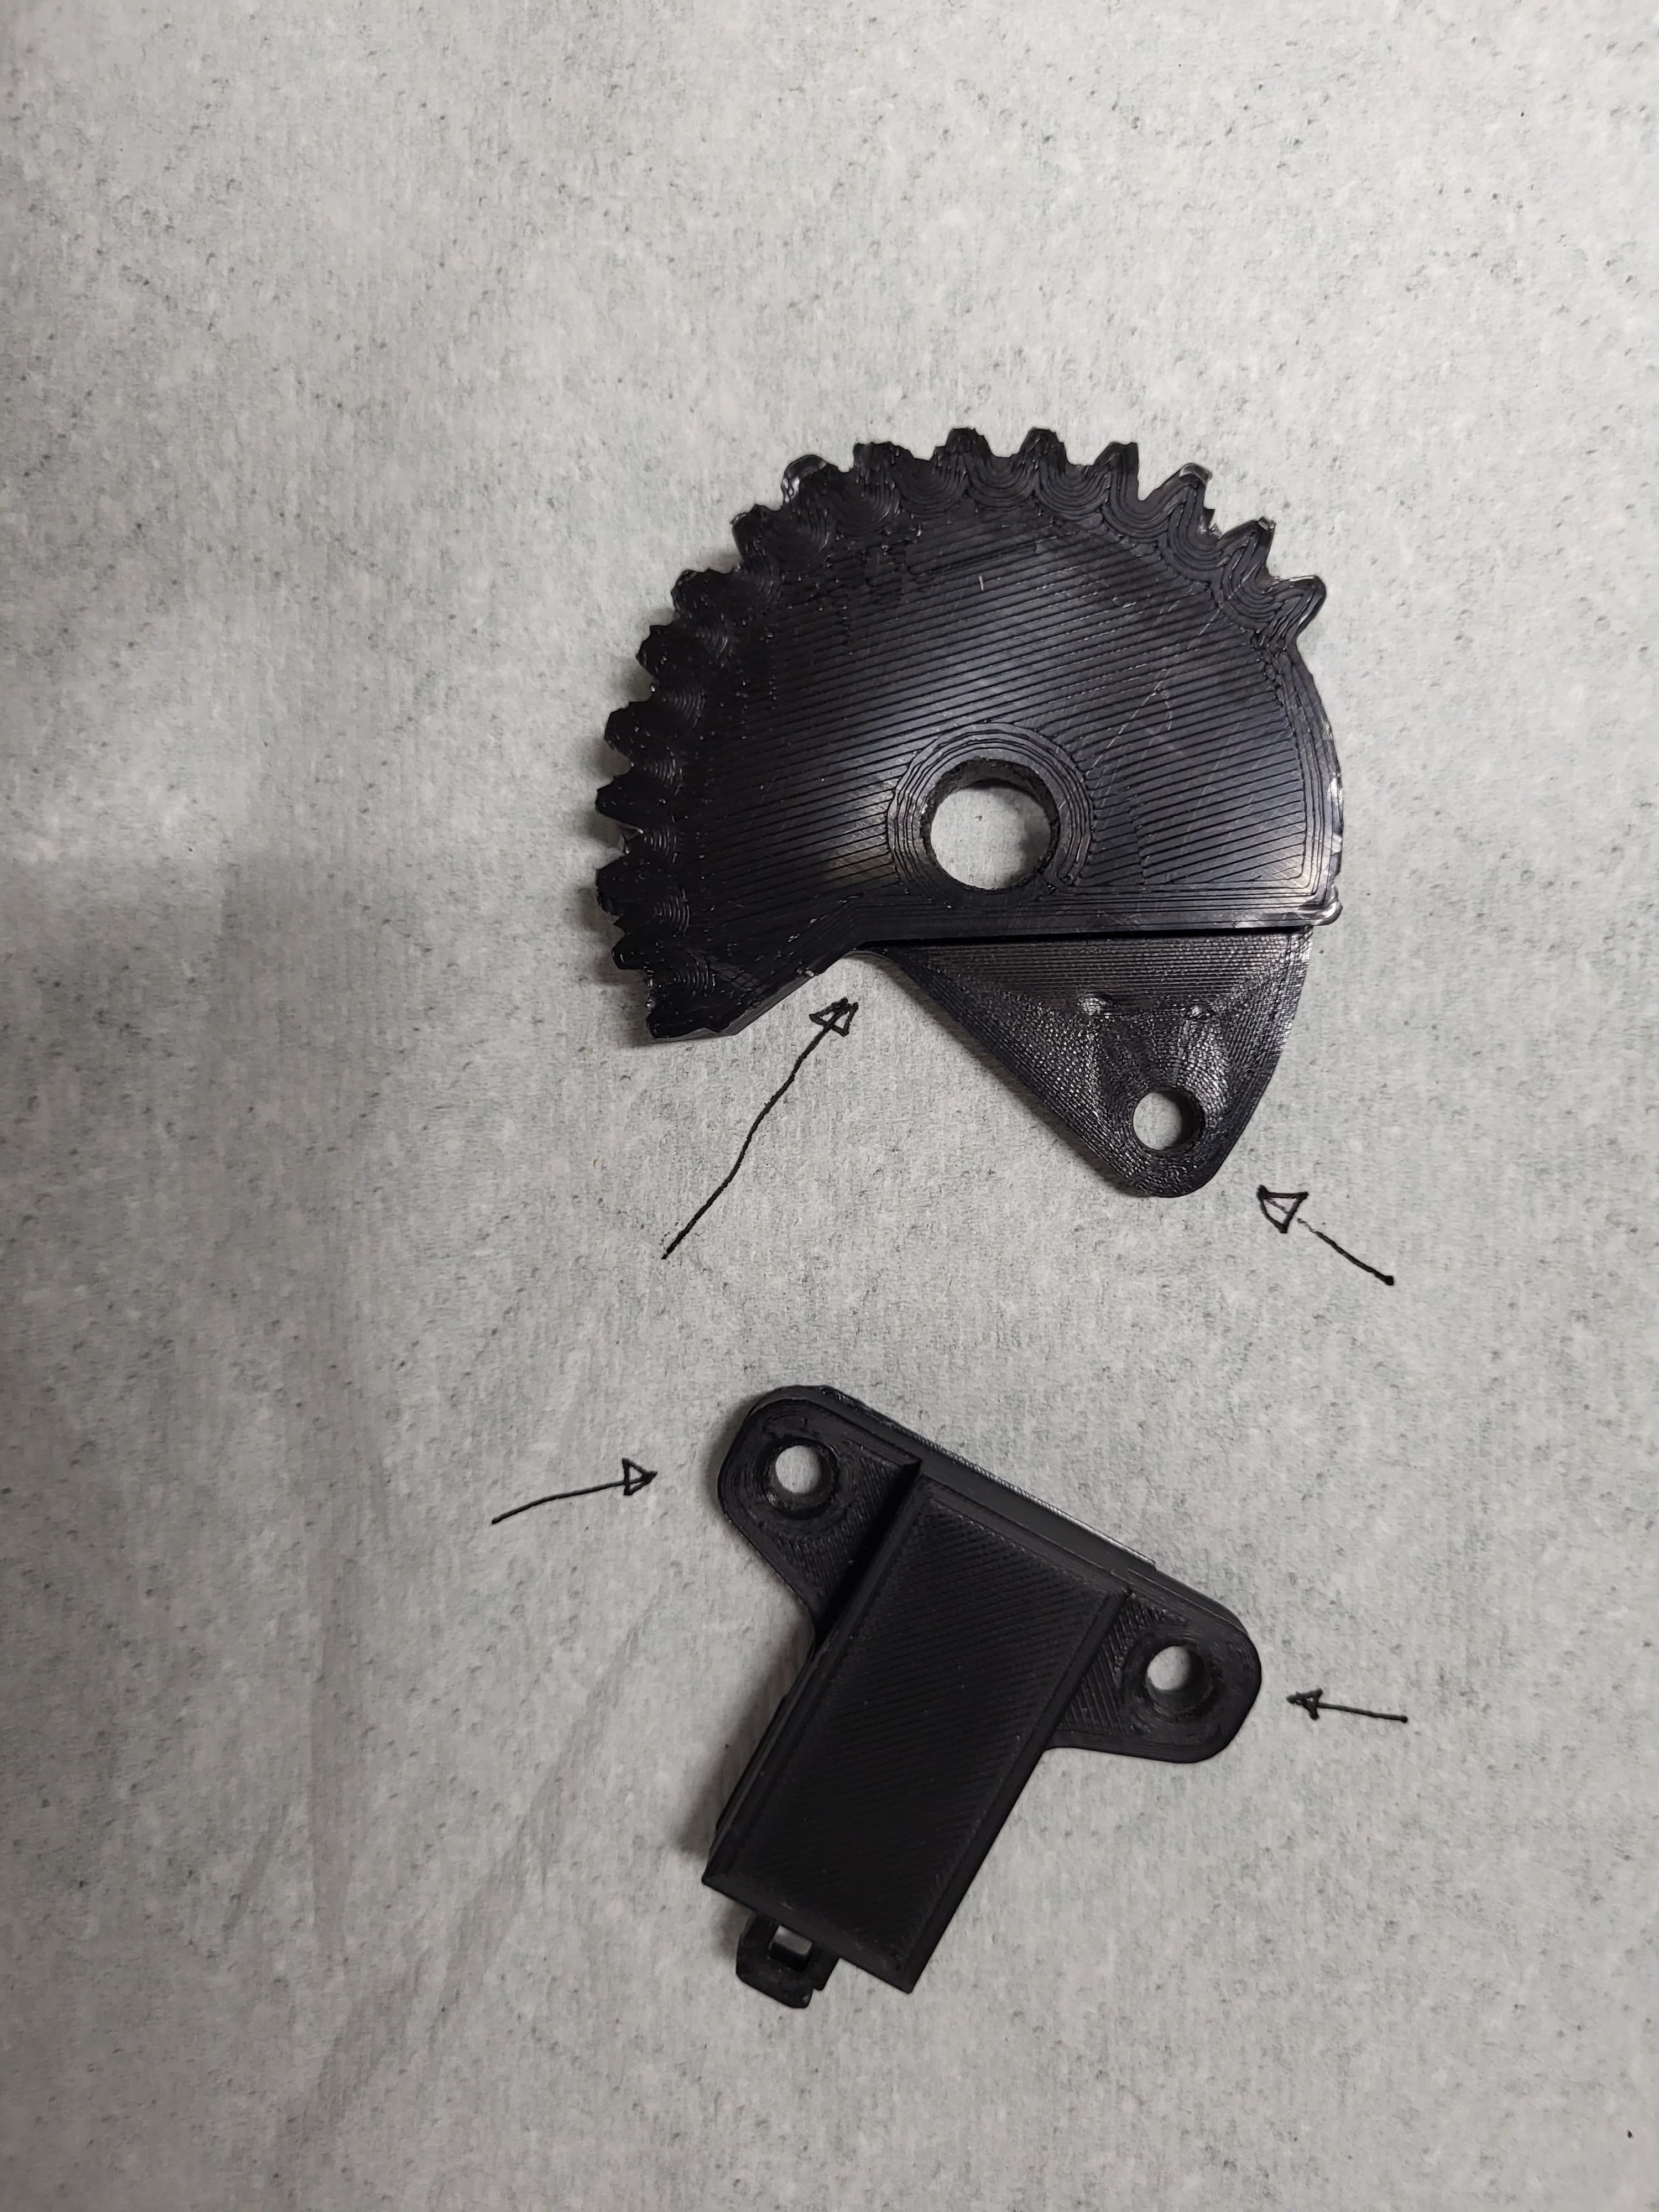
\includegraphics[height=9cm]{img/greifarmtest/prototyp_test_loecher.jpeg}
        \caption{Schrumpfungseffekte 3D-Druck: Alle Löcher sind zu klein}
        \label{fig:hardware_test_loecher}
    \end{minipage}%
    \hfill
    \begin{minipage}[t]{0.45\textwidth}
        \centering
        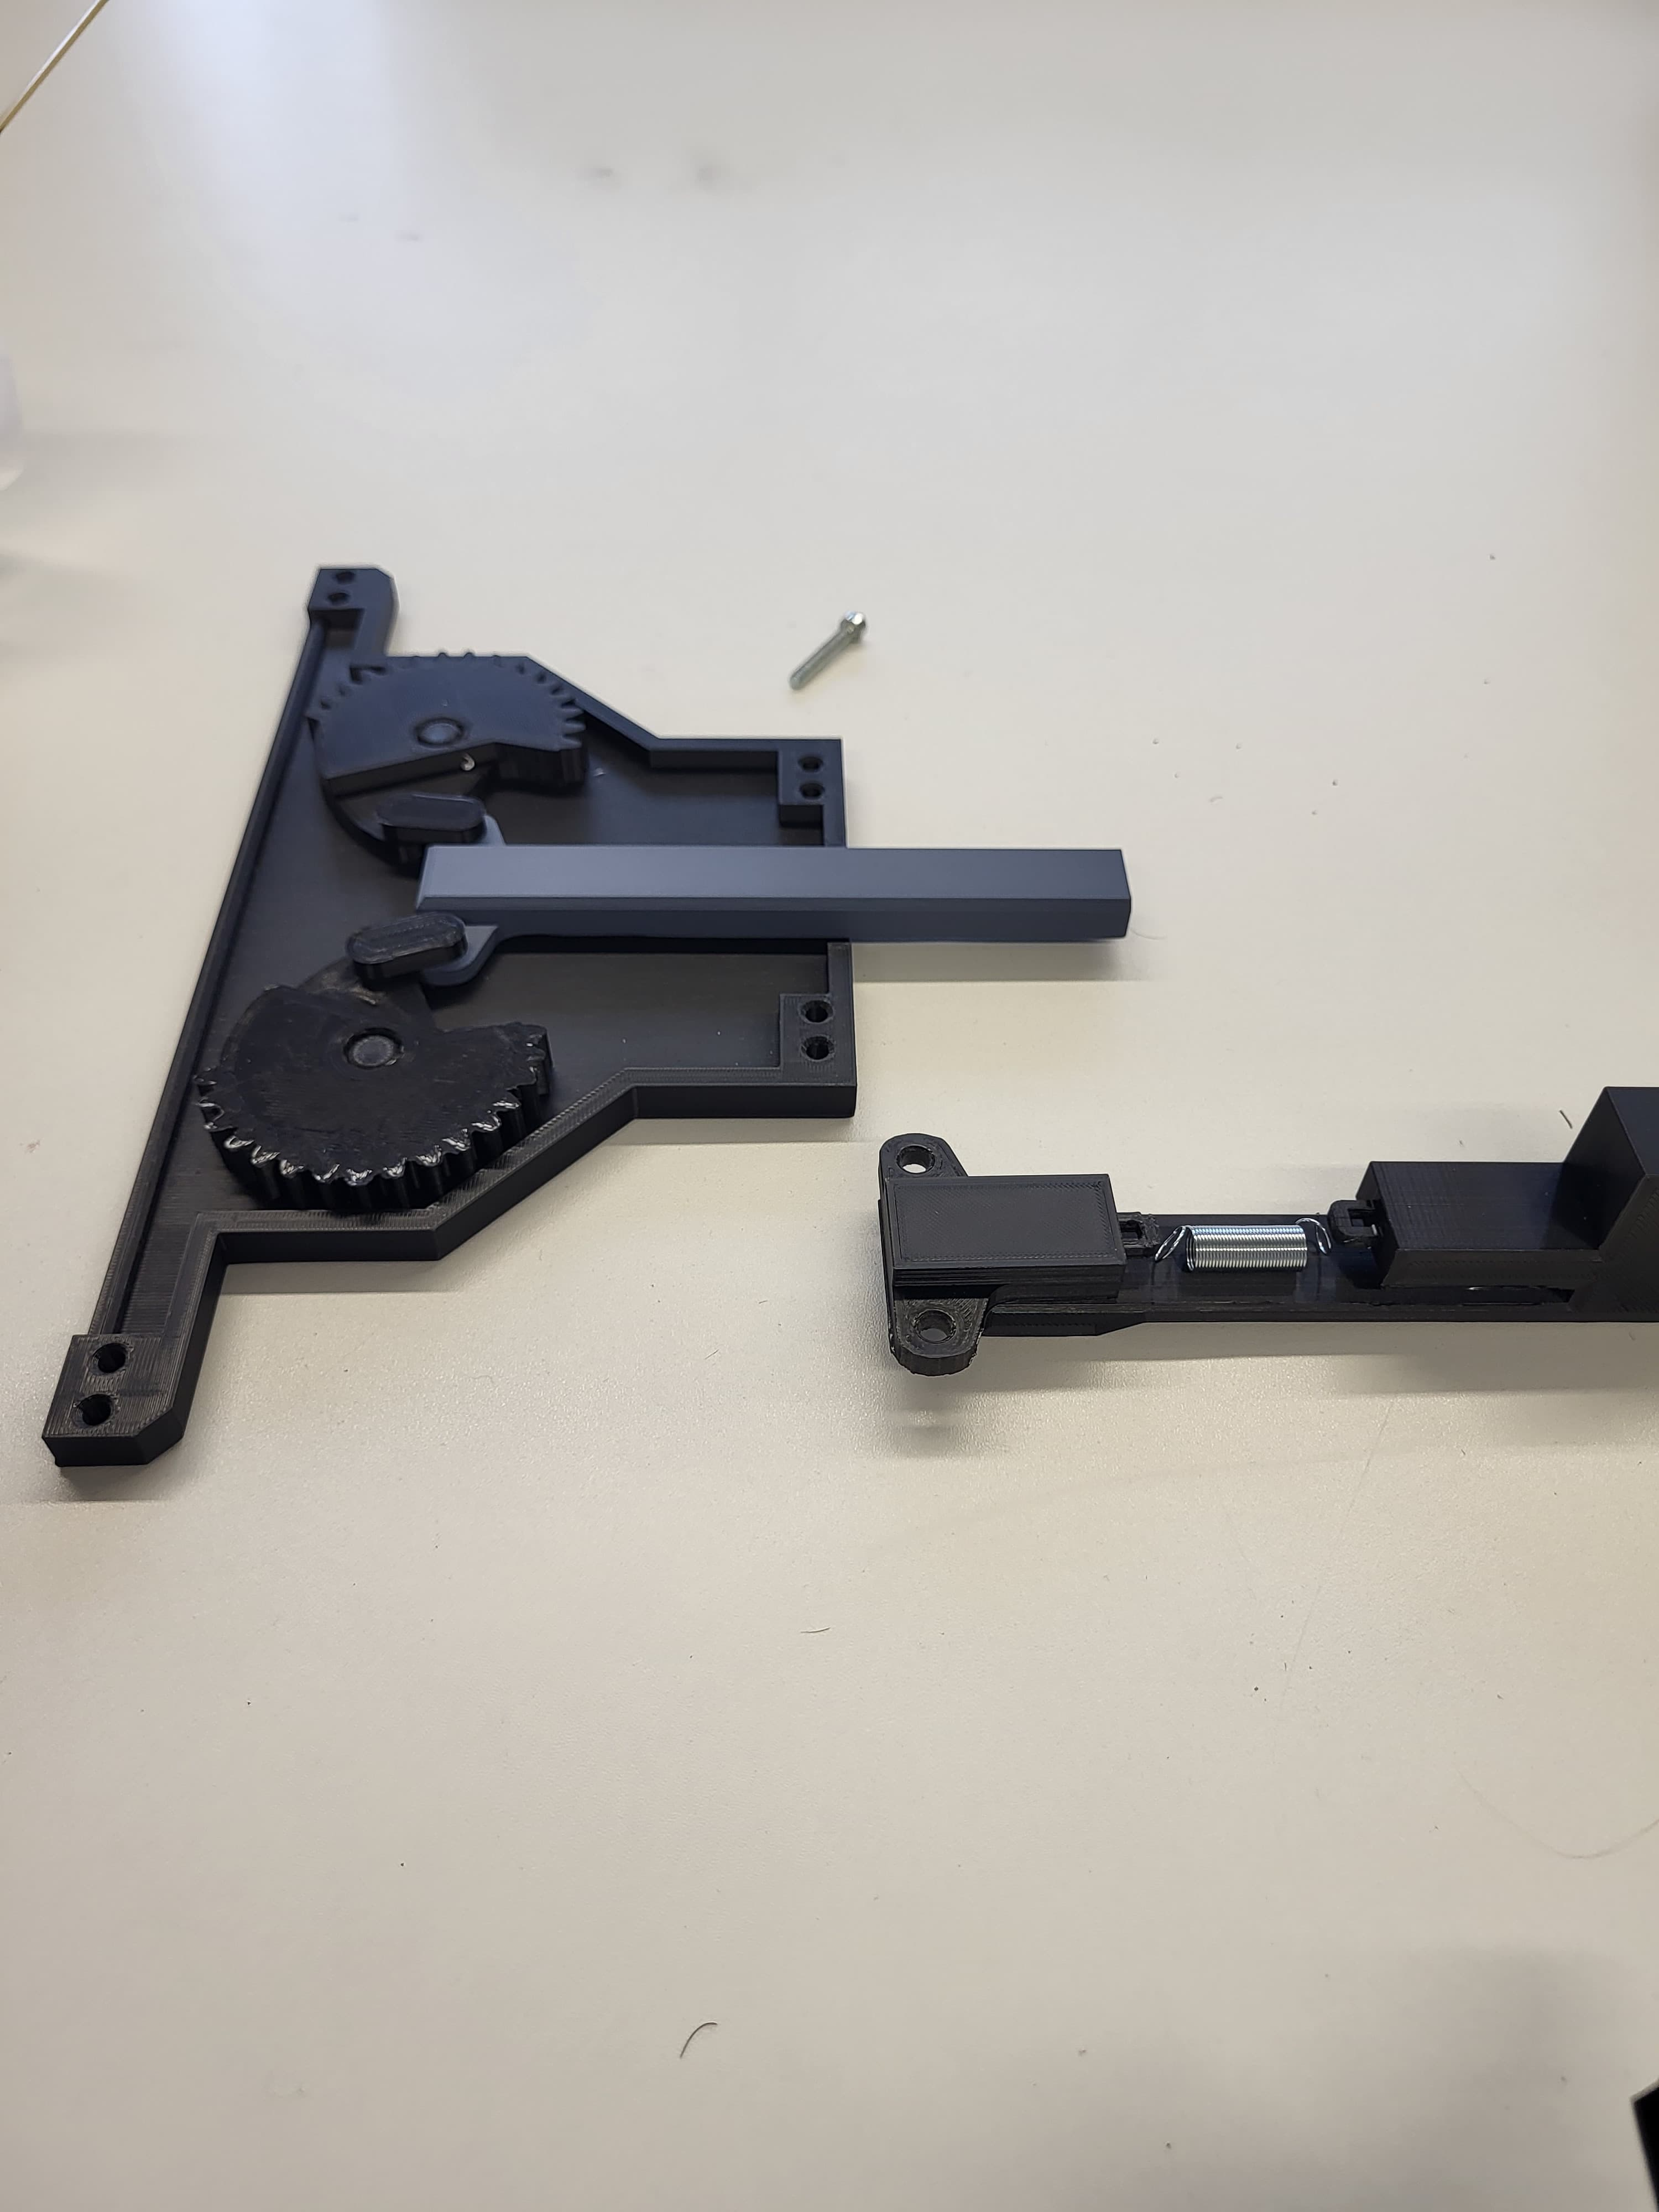
\includegraphics[height=9cm]{img/greifarmtest/prototyp_test_schieber.jpeg}
        \caption{Feder wurde temporär durch einen Schieber ersetzt.}
        \label{fig:hardware_test_schieber}
    \end{minipage}
\end{figure}
\subsubsection{Distanzmessung Hindernis}
Für die Positionierung der Klemmbacken um das Hindernis ist eine Abstandsmessung erforderlich. Im Rahmen der Technologierecherche (siehe Anhang \ref{a2:technologierecherche}) wurden Ultraschallsensoren und \acrshort{tof-sensor}en als mögliche Lösungen identifiziert. Die Wahl fällt auf den Ultraschallsensor, da er bei direkter Sonneneinstrahlung konstante Messwerte liefert. Die durchgeführten Tests zeigten stabile Messungen ab einem Mindestabstand von 3 cm und einer getesteten Reichweite von 30 cm. Der Mindestabstand von 3 cm ist bei der Installation zu berücksichtigen. Der genaue Versuchsaufbau sowie die Messergebnisse sind im Anhang \ref{sec:Distanz_Hindernis} detailliert beschrieben.

\subsubsection{Linienerkennung / Punkterkennung}
Um der Linie zu folgen und den Punkt zu erkennen, ist ein geeigneter Sensor erforderlich. In der Technologierecherche (siehe Anhang \ref{a2:technologierecherche}) wurden zwei mögliche Sensoren identifiziert: ein Farbsensor und ein \gls{ir-fototransistor}. Obwohl der Farbsensor zuverlässig Unterschiede zwischen Boden und Linie erkennt, schied er aufgrund seiner relativ langen Belichtungszeit von 100 ms aus. Er liefert alle 100 ms einen Messwert, was bei einer Geschwindigkeit von 20 cm/s einen Messwert alle 2 cm ergibt. Diese Abtastrate ist nicht ausreichend.

Der \gls{ir-fototransistor} hingegen liefert Messwerte alle 2 ms und erkennt deutliche Unterschiede zwischen den verschiedenen Oberflächen. Darüber hinaus ermöglicht die Analyse der Strichdicke mit mehreren IR-Fototransistoren eine genaue Punkterkennung. Die Details der Versuche und Ergebnisse sind im Anhang \ref{a4:Infrarotfototransistor-Array} dokumentiert.
Das Schema und Layout für den Liniensensor, der mit IR-Dioden und IR-Fototransistoren arbeitet, ist bereits erstellt (siehe Anhang \ref{a4:Schema-Linefollower}).
\end{document}